\documentclass[10pt]{beamer}

\usetheme{metropolis}
\usepackage{appendixnumberbeamer}

\usepackage{booktabs}
\usepackage[scale=2]{ccicons}

\usepackage{pgfplots}
\usepgfplotslibrary{dateplot}

\usepackage{xspace}
\newcommand{\themename}{\textbf{\textsc{metropolis}}\xspace}

\usepackage{amsmath,amssymb,txfonts}

\title{Metropolis}
\subtitle{A modern beamer theme}
\date{\today}
\author{Matthias Vogelgesang}
\institute{Center for modern beamer themes}
\titlegraphic{\hfill
\includegraphics[height=1.5cm]{logo.pdf}}

\begin{document}


\maketitle

\begin{frame}{Table of contents}
  \setbeamertemplate{section in toc}[sections numbered]
  \tableofcontents[hideallsubsections]
\end{frame}

\section{Introduction}

\begin{frame}[fragile]{Metropolis}

  The \themename theme is a Beamer theme with minimal visual noise
  inspired by the \href{https://github.com/hsrmbeamertheme/hsrmbeamertheme}{\textsc{hsrm} Beamer
  Theme} by Benjamin Weiss.

  Enable the theme by loading

  \begin{verbatim}    \documentclass{beamer}
    \usetheme{metropolis}\end{verbatim}

  Note, that you have to have Mozilla's \emph{Fira Sans} font and XeTeX
  installed to enjoy this wonderful typography.
\end{frame}
\begin{frame}[fragile]{Sections}
  Sections group slides of the same topic

  \begin{verbatim}    \section{Elements}\end{verbatim}

  for which \themename provides a nice progress indicator \ldots
\end{frame}

%---------------------------------------------------------------------------------
%-----------------------Taylor-series Method--------------------------------------
%---------------------------------------------------------------------------------
\section{Taylor-series Method}

\begin{frame}{Taylor-series Method}
	we are given:
  $$ r_{i,1}^2=cd_{i,1}=r_{i}-r_{1} $$
  Linearize above equation by Taylor-series expansion and then solve iteratively:
	\begin{itemize}
    \item Compute position deviation
    \item Add position deviation to initial guess
    \item Solve again until deviation is considerably small
  \end{itemize}
  \alert{Convergence is not guaranteed}
\end{frame}


\begin{frame}{Taylor-series Method}
	The position deviation is computed by:
   $$\begin{bmatrix} \Delta x \\ \Delta y \end{bmatrix} = (G_{t}^T Q^{-1} G_{t})^{-1} G_{t}^T Q^{-1} h_{t}$$
  where $h_{t}$ and $G_{t}$ are given as follows
 \begin{align}
    h_{t} &= \begin{bmatrix} r_{2,1} - (r_{2}-r_{1}) \\  r_{3,1} - (r_{3}-r_{1})\\  \quad\\  r_{M,1} - (r_{M}-r_{1}) \end{bmatrix}  \\
    G_{t} &= \begin{bmatrix} (x_{1}-x)/r_{1} - (x_{2}-x)/r_{2} & (y_{1}-y)/r_{1} - (y_{2}-y)/r_{2} \\ (x_{1}-x)/r_{1} - (x_{2}-x)/r_{3} & (y_{1}-y)/r_{1} - (y_{3}-y)/r_{3}\\  \quad\\ (x_{1}-x)/r_{1} - (x_{M}-x)/r_{M} & (y_{1}-y)/r_{1} - (y_{M}-y)/r_{M} \end{bmatrix}
  \end{align}

\end{frame}
%--------------------------end--------------------------------------------------------

%-------------------------------------------------------------------------------------
%------------------------Spherical Interpolation Method-------------------------------
%-------------------------------------------------------------------------------------
\section{Spherical Interpolation Method}

% page 1
\begin{frame}{The Equation-Error Formulation}
  We first map the spatial origin to an arbitrary sensor j, this gives:
  $$ \underline{x}_{j}\triangleq \underline{0}\Longrightarrow \begin{cases} R_{j} &= \ 0 \\ D_{j} &= \ R_{s} \end{cases}$$
  From the Pythagorean theorem, we have:
  $$(R_{s}+d_{ij})^2 = R_{i}^2 - 2\underline{x}_{i}^T \underline{x}_{s} + R_{s}^2 $$
  which is also:
  $$ 0 = R_{i}^2 - d_{ij}^2 -2R_{s}d_{ij} - 2\underline{x}_{i}^T \underline{x}_{s} $$
  \begin{center}
  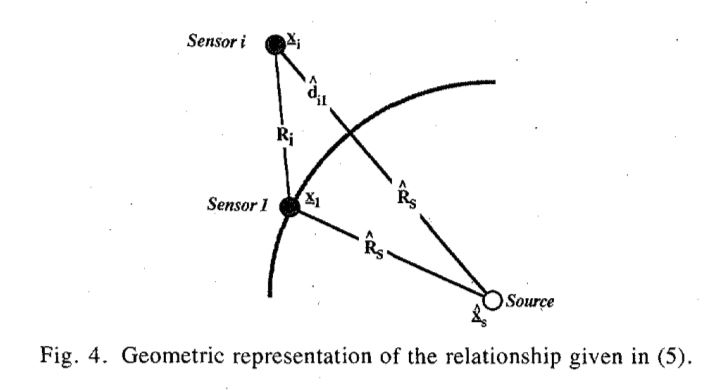
\includegraphics[scale=0.7]{Pythagorean.JPG}
  \end{center}
\end{frame}
% page 2
\begin{frame}{The Equation-Error Fomulation}
  If we take the first sensor as origin, i.e. $j=1$ \\
  As the delays are typically not measured precisely, we introduce "equation error"
  $$ \epsilon_{i} = R_{i}^2 - d_{ij}^2 -2R_{s}d_{ij} - 2\underline{x}_{i}^T \underline{x}_{s} \quad (i=2,3,\ldots,N) $$
  where $\epsilon_{i}$ is to be minimized.
  With N-1 measurements, this equation can be written in matrix notaion:
  $$ \underline{\epsilon} = \underline{\sigma} - 2R_{s}\underline{d} - 2S\underline{x}_{s} $$
  where
  \begin{align*}
    \underline{\sigma}\triangleq \begin{bmatrix} R_{2}^2 - d_{21}^2 \\ R_{3}^2 - d_{31}^2 \\ \vdots \\ R_{N}^2 - d_{N1}^2 \end{bmatrix} \qquad
    \underline{d}\triangleq \begin{bmatrix} d_{21}\\ d_{31} \\ \vdots \\ d_{N1} \end{bmatrix} \qquad
    \textbf{S} \triangleq \begin{bmatrix} x_2 & y_2 \\x_3 & y_3\\ \vdots & \vdots \\ x_N & y_N \end{bmatrix}
  \end{align*}
\end{frame}







\begin{frame}{Font feature test}
  \begin{itemize}
    \item Regular
    \item \textit{Italic}
    \item \textsc{Small Caps}
    \item \textbf{Bold}
    \item \textbf{\textit{Bold Italic}}
    \item \textbf{\textsc{Bold Small Caps}}
    \item \texttt{Monospace}
    \item \texttt{\textit{Monospace Italic}}
    \item \texttt{\textbf{Monospace Bold}}
    \item \texttt{\textbf{\textit{Monospace Bold Italic}}}
  \end{itemize}
\end{frame}

\begin{frame}{Lists}
  \begin{columns}[T,onlytextwidth]
    \column{0.33\textwidth}
      Items
      \begin{itemize}
        \item Milk \item Eggs \item Potatoes
      \end{itemize}

    \column{0.33\textwidth}
      Enumerations
      \begin{enumerate}
        \item First, \item Second and \item Last.
      \end{enumerate}

    \column{0.33\textwidth}
      Descriptions
      \begin{description}
        \item[PowerPoint] Meeh. \item[Beamer] Yeeeha.
      \end{description}
  \end{columns}
\end{frame}
\begin{frame}{Animation}
  \begin{itemize}[<+- | alert@+>]
    \item \alert<4>{This is\only<4>{ really} important}
    \item Now this
    \item And now this
  \end{itemize}
\end{frame}
\begin{frame}{Figures}
  \begin{figure}
    \newcounter{density}
    \setcounter{density}{20}
    \begin{tikzpicture}
      \def\couleur{alerted text.fg}
      \path[coordinate] (0,0)  coordinate(A)
                  ++( 90:5cm) coordinate(B)
                  ++(0:5cm) coordinate(C)
                  ++(-90:5cm) coordinate(D);
      \draw[fill=\couleur!\thedensity] (A) -- (B) -- (C) --(D) -- cycle;
      \foreach \x in {1,...,40}{%
          \pgfmathsetcounter{density}{\thedensity+20}
          \setcounter{density}{\thedensity}
          \path[coordinate] coordinate(X) at (A){};
          \path[coordinate] (A) -- (B) coordinate[pos=.10](A)
                              -- (C) coordinate[pos=.10](B)
                              -- (D) coordinate[pos=.10](C)
                              -- (X) coordinate[pos=.10](D);
          \draw[fill=\couleur!\thedensity] (A)--(B)--(C)-- (D) -- cycle;
      }
    \end{tikzpicture}
    \caption{Rotated square from
    \href{http://www.texample.net/tikz/examples/rotated-polygons/}{texample.net}.}
  \end{figure}
\end{frame}
\begin{frame}{Tables}
  \begin{table}
    \caption{Largest cities in the world (source: Wikipedia)}
    \begin{tabular}{@{} lr @{}}
      \toprule
      City & Population\\
      \midrule
      Mexico City & 20,116,842\\
      Shanghai & 19,210,000\\
      Peking & 15,796,450\\
      Istanbul & 14,160,467\\
      \bottomrule
    \end{tabular}
  \end{table}
\end{frame}
\begin{frame}{Blocks}
  Three different block environments are pre-defined and may be styled with an
  optional background color.

  \begin{columns}[T,onlytextwidth]
    \column{0.5\textwidth}
      \begin{block}{Default}
        Block content.
      \end{block}

      \begin{alertblock}{Alert}
        Block content.
      \end{alertblock}

      \begin{exampleblock}{Example}
        Block content.
      \end{exampleblock}

    \column{0.5\textwidth}

      \metroset{block=fill}

      \begin{block}{Default}
        Block content.
      \end{block}

      \begin{alertblock}{Alert}
        Block content.
      \end{alertblock}

      \begin{exampleblock}{Example}
        Block content.
      \end{exampleblock}

  \end{columns}
\end{frame}
\begin{frame}{Math}
  \begin{equation*}
    e = \lim_{n\to \infty} \left(1 + \frac{1}{n}\right)^n
  \end{equation*}
\end{frame}
\begin{frame}{Line plots}
  \begin{figure}
    \begin{tikzpicture}
      \begin{axis}[
        mlineplot,
        width=0.9\textwidth,
        height=6cm,
      ]

        \addplot {sin(deg(x))};
        \addplot+[samples=100] {sin(deg(2*x))};

      \end{axis}
    \end{tikzpicture}
  \end{figure}
\end{frame}
\begin{frame}{Bar charts}
  \begin{figure}
    \begin{tikzpicture}
      \begin{axis}[
        mbarplot,
        xlabel={Foo},
        ylabel={Bar},
        width=0.9\textwidth,
        height=6cm,
      ]

      \addplot plot coordinates {(1, 20) (2, 25) (3, 22.4) (4, 12.4)};
      \addplot plot coordinates {(1, 18) (2, 24) (3, 23.5) (4, 13.2)};
      \addplot plot coordinates {(1, 10) (2, 19) (3, 25) (4, 15.2)};

      \legend{lorem, ipsum, dolor}

      \end{axis}
    \end{tikzpicture}
  \end{figure}
\end{frame}
\begin{frame}{Quotes}
  \begin{quote}
    Veni, Vidi, Vici
  \end{quote}
\end{frame}

{%
\setbeamertemplate{frame footer}{My custom footer}
\begin{frame}[fragile]{Frame footer}
    \themename defines a custom beamer template to add a text to the footer. It can be set via
    \begin{verbatim}\setbeamertemplate{frame footer}{My custom footer}\end{verbatim}
\end{frame}
}

\begin{frame}{References}
  Some references to showcase [allowframebreaks] \cite{knuth92,ConcreteMath,Simpson,Er01,greenwade93}
\end{frame}

\section{Conclusion}

\begin{frame}{Summary}

  Get the source of this theme and the demo presentation from

  \begin{center}\url{github.com/matze/mtheme}\end{center}

  The theme \emph{itself} is licensed under a
  \href{http://creativecommons.org/licenses/by-sa/4.0/}{Creative Commons
  Attribution-ShareAlike 4.0 International License}.

  \begin{center}\ccbysa\end{center}

\end{frame}

\begin{frame}[standout]
  Questions?
\end{frame}

\appendix

\begin{frame}[fragile]{Backup slides}
  Sometimes, it is useful to add slides at the end of your presentation to
  refer to during audience questions.

  The best way to do this is to include the \verb|appendixnumberbeamer|
  package in your preamble and call \verb|\appendix| before your backup slides.

  \themename will automatically turn off slide numbering and progress bars for
  slides in the appendix.
\end{frame}

\begin{frame}[allowframebreaks]{References}

  \bibliography{demo}
  \bibliographystyle{abbrv}

\end{frame}

\end{document}
